%% use article style

\documentclass[12pt]{article}
\usepackage{amsmath,amssymb,amsthm,amsfonts}
\usepackage{graphicx}
\title{A new look at Pompeiu Triangles}
\begin{document}
\maketitle
\section{Introduction}
Ptolemey's theorem states that if $ABCD$ is a cyclic quadrilateral, then $AB\cdot CD+BC\cdot DA=AC\cdot BD$. When $D$ does not belong to the circumcircle of $ABC$, then the following inequality holds: $AB\cdot CD+BC\cdot DA>AC\cdot BD$. If $ABC$ is an equilateral triangle (and using $P$ instead of $D$ to denote the fourth point), then $PC+PA \geq PB$. This is because $AB=BC=CA$ and $P$ does not belong to the circumcircle of $ABC$. Given that the inequality above (called the triangle inequality) holds, one can construct a triangle with sides $PA$, $PB$ and $PC$.  Such a triangle is called a Pompeiu triangle. The name comes from the Romanian mathematician Dimitrie Pompeiu, who studied these triangles in 1929. An interesting property of Pompeiu triangles is that their areas can be calculated using elementary geometry. Moreover, their areas are related to other geometric properties. In this paper, we will present a new way of deriving the formula to 
calculate the area of a Pompeiu triangle. The derivation involves circular inversions. We also derive a formula to relate this area to the distance of point D to the circumcircle of $ABC$. A derivation based on inversions was presented by Benyi and Casu (2009). However, the derivation presented here is simpler and more elegant. 

\section{Circular inversions}
Inversions are a powerful tool in geometry. They are used to prove many theorems. In this section, we will present the basic properties of inversions. We will also present a formula to calculate the area of a triangle using inversions.

In plane geometry the inverse of a point $P$ with respect to a reference circle with center $O$ and radius $k$ is a point $P'$, lying on the ray from $O$ through $P$ such that

\begin{equation}
OP\cdot OP'=k^2
\label{eq:inversion}
\end{equation}

A remarkable property of inversions is that they transform circles that go through the center of inversion into straight lines. This is a property that we will use in this paper to derive the formula for the area of a Pompeiu triangle. For a proof of this property, see https://artofproblemsolving.com/wiki/
index.php/Circular\_Inversion.
Another property that we will use is that if $A'$ and $B'$ are the inverses of points $A$ and $B$ then 

\begin{equation}
{A'B'}={AB}\frac{k^2}{OA\cdot OB}
\label{eq:inversion2}
\end{equation}

\section{The area of a Pompeiu triangle}

%% insert figure 1 here
\subsection{Some preliminary results}
For a given equilateral triangle $\Delta ABC$, we can apply an inversion with respect to a reference circle with center $A$ and radius $k$, and transform points $A$ and $B$ into point $A'$ and $B'$. A point $P$ interior to triangle $\Delta ABC$ is transformed into $P'$, which is exterior to triangle $\Delta AB'C'$. This is illustrated in Figure \ref{fig:pompeiuTriangles1}. It may be noticed in this figure that the area of $\Delta B'P'C'$ can be determined from the areas of triangles $\Delta AB'P'$, $\Delta AP'C'$ and $\Delta AB'C'$.  More specifically, if we denote the area of any given triangle $\Delta ABC$ by $S(ABC)$, then

\begin{equation}
S(B'P'C')=S(AB'P')+S(AP'C')-S(AB'C')
\label{eq:area1}
\end{equation}

To relate equation ref{eq:area1} to the area of a Pompeiu triangle, we need to express the areas of triangles $\Delta B'P'C'$, $\Delta AB'P'$, $\Delta AP'C'$ and $\Delta AB'C'$ in terms of the untransformed distances among points $A$,$B$,$C$ and $P$.

According to equation \ref{eq:inversion2}, $B'C'=BC\frac{k^2}{AB\cdot AC}$, $B'P'=BP\frac{k^2}{AB\cdot AP}$ and $P'C'=PC\frac{k^2}{AP\cdot AC}$. 
However, $AB$=$BC$=$AC$=$a$. Therefore, $B'C'=\frac{k^2}{a}$, $B'P'=BP\frac{k^2}{a\cdot AP}$ and $P'C'=PC\frac{k^2}{a\cdot AP}$. Rewriting $B'C'$ as $B'C'=PA \frac{k^2}{a \cdot AP}$, we can notice that the sides of triangle $\Delta B'P'C'$ are proportional to the sides of triangle formed with segments $PA$, $PB$, $PC$. The scale factor is $\frac{k^2}{a \cdot AP}$. Therefore, the area of $\Delta B'P'C'$ is proportional to the area of Pompeiu triangle $(PA,PB,PC)$. More specifically, $S(B'P'C')=S(P(PA,PB,PC))(\frac{k^2}{a PA})^2$.

\begin{figure}[h]
\centering
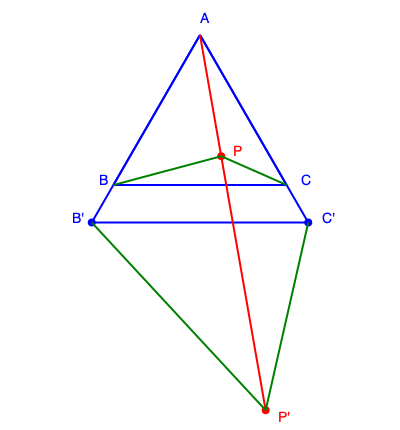
\includegraphics[width=0.75\textwidth]{pompeiuTriangle.png}
\caption{A Pompeiu triangle}
\label{fig:pompeiuTriangles1}
\end{figure}

To express the area of triangles $\Delta AB'P'$ as a function of $S(ABP)$, we can use $S(AB'P')=\frac {AB'\cdot AP' \cdot \sin(B'AP')}{2}$=
$\frac{1}{2} \cdot \frac {k^2} {AB} \cdot \frac {k^2}{AP} \cdot \sin(BAP)$=$\frac {k^4} {AB^2 PA^2} \cdot \frac {AB \cdot AP \cdot \sin(BAP)} {2}$=$\frac {k^4}{a^2 PA^2} S(ABP)$. Similarly, $S(AP'C')=\frac {k^4}{a^2 PA^2} S(APC)$. 

On the other hand, $S(AB'C')=\frac {k^4}{a^4}S(ABC)$.  Therefore,

\begin{equation}
    S(P(PA,PB,PC))=S(ABP)+ S(APC)-\frac{PA^2}{a^2}S(ABC)
    \label{eq:area2}
\end{equation}

As $S(P(PA,PB,PC))$ depends on $S(ABP)$, $S(APC)$, $S(ABC)$ and $MA$, it follows that a simple but general way of expressing $S(ABP)$, $S(APC)$, and $AP$ in terms of the side of the equilateral triangle $a$ and $MA$ needed.  This can be accomplished through elementary vector analysis (Weatherburn, 1926).

\subsection{Elements of vector analysis}

The theory of vectors was developed in the second half of the 18th in response to the need to rigorously and efficiently investigate problems in physics. As many physically properties such as forces, velocities, 3D displacements, etc. can be represented by vectors, cannot be described by single numbers (scalars), the theory of vectors was developed to provide a mathematical framework to study these properties. For example, a force cannot be described by a single number related to its magnitude because its direction is important as well. Similarly, position of a point relative to another cannot be described by the distance between them because the orientation relative to a given direction is a defining factor as well. However, the direction defined as value of an angle is not useful because it precludes the use of algebraic operations such as addition and subtraction. Therefore, instead of angular values, vectors rely on the concept of decomposition along two independent directions.  To describe the decomposition of a vector along two independent, we need to first define vectors and the addition of two vectors. In geometry, vectors are just directed segments.  For example, vector $\vec {AB}$ in Figure \ref{fig:vectors} is just segment $AB$ oriented from $A$ to $B$. The addition of two vectors is defined as the vector obtained by placing the second vector at the end of the first vector. For example, the sum of vectors $\vec {AF}$ and $\vec {FB}$ is vector $\vec {AC}$.  Equation 
\begin{equation}
\vec {AB}=\vec {AF} + \vec {FB}
\label{eq:vectorAddition}
\end{equation}
is called the triangle law of addition and is true irrespective of where $F$ is located in the plane. However because $F$ is on line $d1$ and $FB$ is parallel to line $d2$, we can say that vectors $\vec{AF}$ and $\vec{FB}$ are the components of $\vec{AB}$ along directions $d1$ and $d2$.  The decomposition of a vector along two independent directions is unique.  This means that if we know the decomposition of a vector along two independent directions, we can determine the vector.  Note that a different vector, i.e. $\vec{AC}$ with same magnitude as $\vec{AB}$, but different direction, has different components on $d1$ and $d2$. In short, to define a vector, we need to specify its components along two independent (arbitrary but defined) directions.  The determination of a vector from its components and the inverse operation are trivial.

In addition to decomposition and vector addition, another important operation is its multiplication by a scalar.  The multiplication of a vector by a scalar is defined as the vector obtained by multiplying the magnitude of the vector by the scalar and keeping the direction of the vector.  For example, the vector $2\vec{AB}$ is twice as long as $\vec{AB}$ and has the same direction.  If we multiply by a negative scalar, in addition to changing the magnitude of the vector, we also invert its direction. 

An extremely important vector operation is the dot product between two vectors $\vec{a}$ and $\vec{b}$, defined as 
\begin{equation}
\vec{a}\cdot\vec{b}=|a||b|\cos(\theta)
\label{eq:dotProduct}
\end{equation}
where $|a|$ and $|b|$ are the magnitudes of vectors $\vec{a}$ and $\vec{b}$ and $\theta$ is the angle between them.  While extremely important, the significance of the dot product is not immediately obvious. A major reason for the introduction of the dot product is its utility in deriving the components of a vector with respect to two new directions $d1_{new}$ and $d2_{new}$ from its components with respect to current directions $d1$ and $d2$.  Another benefit is in easily calculating distances, as it will be obvious in the article.

\begin{figure}[h]
    \centering
    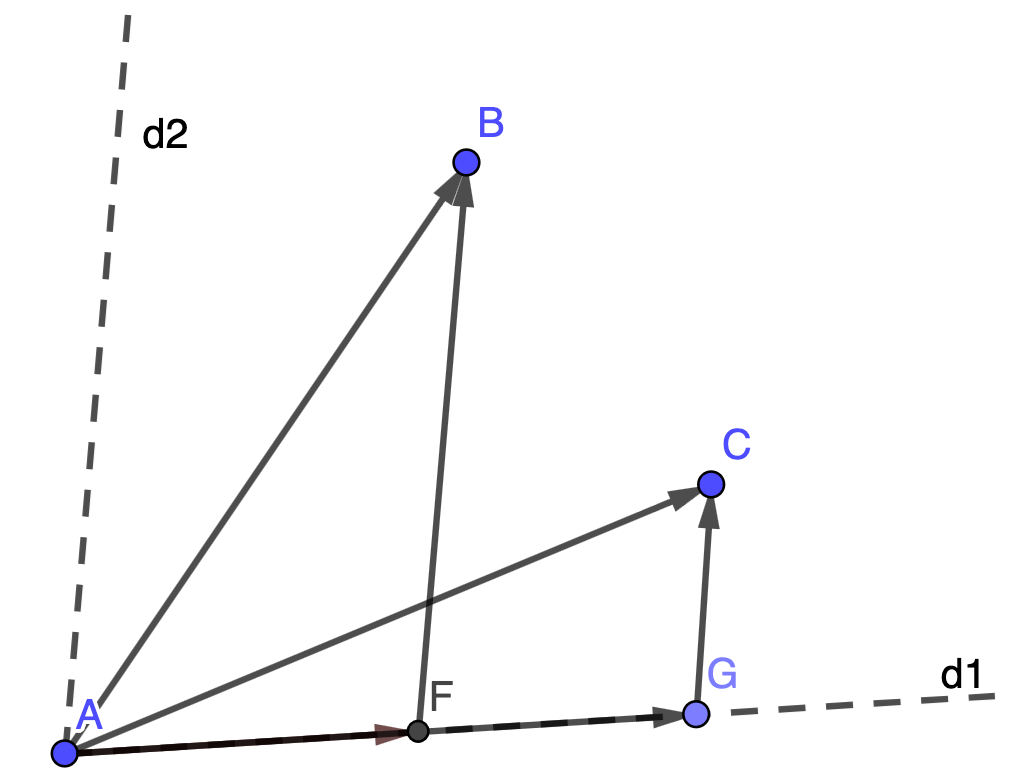
\includegraphics[width=0.75\textwidth]{Vectors.png}
    \caption{Two vectors and their decompositions.}
    \label{fig:vectors}
    \end{figure}

Although not directly used in this article the cross product between two vectors $\vec{a}$ and $\vec{b}$ is also important. We mention it here without a definition.

A concept that is used in the article to derive various formula used in the simplification of Equation \ref{eq:area2} is that of centroid. The centroid of a system of points $P_1$, $P_2$, ..., $P_n$ associated with masses $m_1$, $m_2$, ..., $m_n$ is the point $G$ defined by the equation
\begin{equation}
\vec{OG}=\frac{1}{\sum_{i=1}^n m_i}\sum_{i=1}^{n}m_i\vec{OP_i}
\label{eq:centroid}
\end{equation}
where $G$ is the centroid location and $O$ is the origin of the coordinate system.

It can be proven that the location of $G$ does not depend on that of $O$ (Weatherburn, 1926).

\subsection{Some useful formulas}
Consider an arbitrary triangle $ABC$ to which we attach masses $k_1$, $k_2$ and $k_3$. According to Eq. \ref{eq:centroid} when the origin is point $A$, the centroid of the system consistent of masses $k_2$ and $k_3$ is

\begin{equation}
\vec{AD}=\frac{1}{k_2+k_3}(k_2\vec{AB}+k_3\vec{AC})
\end{equation}
If we denote the centroid of the system of masses $k_1$, $k_2$ and $k_3$ by $P$, then

\begin{equation}
\vec{AP}=\frac{1}{k_1+k_2+k_3}(k_2\vec{AB}+k_3\vec{AC})
\label{eq:centroid2}
\end{equation}
Note that $\vec{AP}$ and $\vec{AD}$ are both proportional to $k_2 \vec{AB}+ k_3\vec{AC}$.  They have the same origin and same direction, but they have different magnitudes (on lengths). The ratio of their magnitudes is $\frac{k_1+k_2+k_3}{k_2+k_3}$.  Therefore, $P$ is located on $AD$ at a distance $\frac{k_2+k_3}{k_1+k_2+k_3} AD$ from $A$.  Moreover, $P$ is located at a distance of $\frac{k_1}{k_1+k_2+k_3} AD$ from $D$. It follows that the area of triangle $\Delta BPC$ is $\frac{k_1}{k_1+k_2+k_3} S(ABC)$. Similarly, the area of triangle $\Delta APC$ is $\frac{k_2}{k_1+k_2+k_3} S(ABC)$ and the area of triangle $\Delta APB$ is $\frac{k_3}{k_1+k_2+k_3} S(ABC)$.  

The converse is also true. That is, given a point $P$ in the interior of a triangle, there are masses $k_1$, $k_2$, $k_3$ that can be attached to points $A$, $B$, $C$ such that the centroid of the system is $P$.  The masses are given by $k_1=\frac{S(BPC)}{S(ABC)}$, $k_2=\frac{S(APC)}{S(ABC)}$ and $k_3=\frac{S(APB)}{S(ABC)}$.

\subsection{Derivation of the formula for the area of a Pompeiu triangle}
Equation \ref{eq:area2} can be then rewritten as

\begin{equation}
S(P(PA,PB,PC))=S(ABC)\left(\frac{k_2+k_3}{k_1+k_2+k_3}-\frac{PA^2}{a^2}\right)
\label{eq:area3}
\end{equation}

To further simplify Eq. \ref{eq:area3}, we can calculate the dot product of $\vec{AP}$ with itself.  This is given by
\begin{equation}
\vec{AP}\cdot\vec{AP}=\frac{1}{(k_1+k_2+k_3)^2}(k_2\vec{AB}+k_3\vec{AC})\cdot(k_2\vec{AB}+k_3\vec{AC})
\label{eq:dotProduct2}
\end{equation}
Expanding the dot product in Eq. \ref{eq:dotProduct2} and using the fact that $\vec{AB}\cdot\vec{AB}=a^2$, $\vec{AC}\cdot\vec{AC}=a^2$ and $\vec{AB}\cdot\vec{AC}=\frac{a^2}{2}$, we obtain
\begin{equation}
AP^2=\frac{1}{(k_1+k_2+k_3)^2}(k_2^2a^2+k_3^2a^2+k_2k_3a^2)
\label{eq:dotProduct3}
\end{equation}
\begin{figure}
\centering
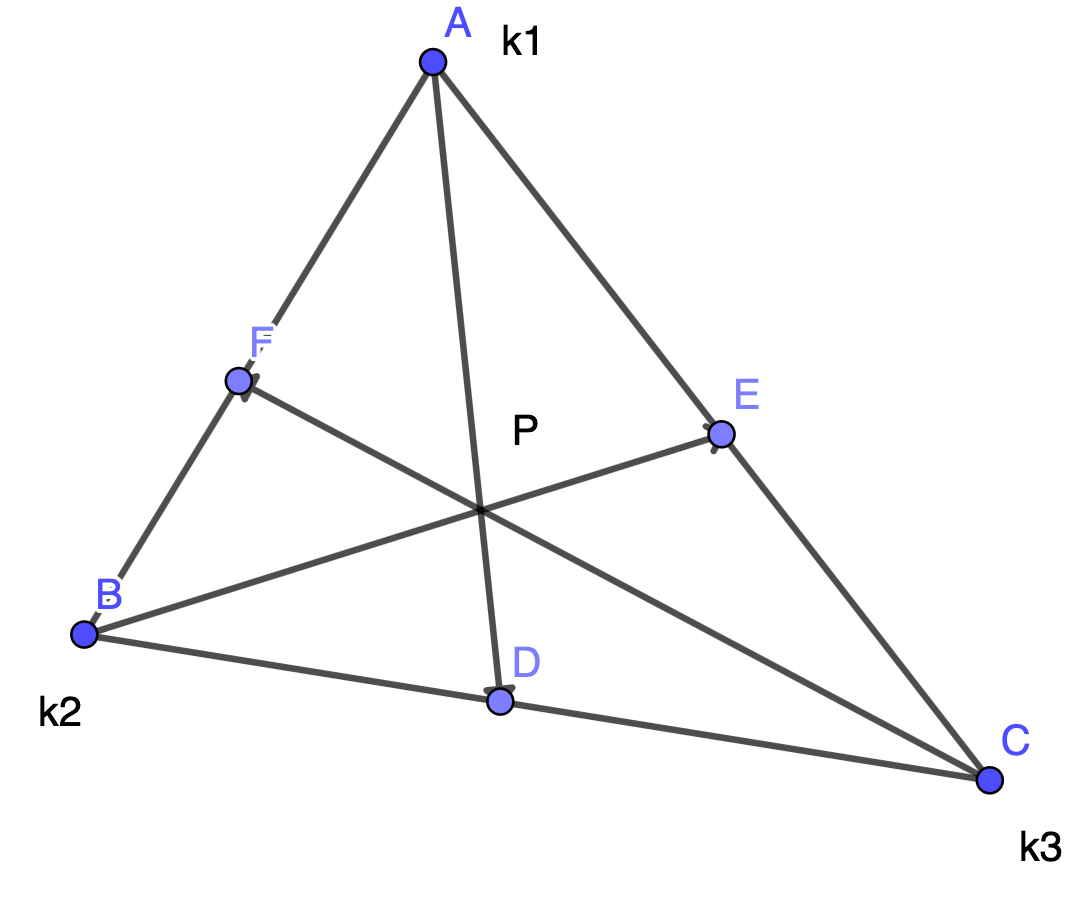
\includegraphics[width=0.75\textwidth]{centroid.png}
\caption{An arbitrary triangle $ABC$ with masses $k_1$, $k_2$, $k_3$ attached at points $A$, $B$, $C$.}
\label{fig:centroid}
\end{figure}

Therefore, Eq. \ref{eq:area3} can be rewritten as
\begin{equation}
S(P(PA,PB,PC))=S(ABC)\left(\frac{k_2+k_3}{k_1+k_2+k_3}-\frac{k_2^2+k_3^2+k_2k_3}{(k_1+k_2+k_3)^2}\right)
\label{eq:area4}
\end{equation}
or
\begin{equation}
S(P(PA,PB,PC))=S(ABC)\left(\frac{k_1k_2+k_1k_3+k_2k_3}{(k_1+k_2+k_3)^2}\right)
\label{eq:area5}
\end{equation}
Benyi and Casu (2009) derived a formula similar Eq. \ref{eq:area5} also relying on inversions. However, they do not use vector geometry and the steps from Eq. \ref{eq:area2} to the final form are significantly more algebraic in nature. Moreover, the algebraic steps are not as intuitive as the vector geometry steps presented here and do not enable the derivation of the formula for the distance of point $P$ to the circumcircle of $ABC$.

\subsection{A remarkable property of Pompeiu triangles}
In Andreescu et al. (2009), the reader is asked to find the geometric locus of points P that have the same areas. The original author of the problem is unknown, but the problem is believed to have been known for quite a while before it was published in the book. 

\section{Reference}
Andreescu, T., Gelca, R. and Saul, M., 2009. Mathematical olympiad challenges (Vol. 216). Boston, MA: Birkhäuser.
Bényi, Á. and Caşu, L., 2009. Pompeiu's Theorem Revisited. The College Mathematics Journal, 40(4), pp.252-258.
Weatherburn, Charles Ernest. Elementary Vector Analysis: With application to geometry and physics. Bell and Sons, 1926.
\end{document}